\documentclass[12pt]{article}
\usepackage{fullpage,amsfonts,amsmath,graphicx,verbatim,parskip,color,mdframed}
\usepackage[left=2cm,top=2cm,right=2cm,bottom=2cm,head=2cm,foot=1cm]{geometry}
\usepackage{notes}

\usepackage{notes}
\newcommand{\solution}{\textbf{Solution: }}
\renewcommand{\P}{\Pr}

\title{Machine Learning}

\begin{document}

\maketitle

\begin{itemize}
\item $n$ sample points $x_i \in \R^d$, $i = 1, \ldots, n$
\item $d = 2$ where not stated.
\end{itemize}

\section*{Classification}

A \textbf{decision boundary} is a curve separating the plane (sample space)
into two regions.

Some classifiers involve a \textbf{decision function} $f$, in which case
$f(\x) = 0$ describes the decision boundary.

A \textbf{linear classifier} uses a linear decision function
$f(x) = \w \cdot \x + \alpha$. This is scalar-valued: it's a plane over
the plane (sample space). Its intersection defines a linear decision boundary.

In $d$-dimensions the decision boundary is a hyperplane
($(d-1)$-dimensional). This still separates the sample space into two regions.

\textbf{Example:} $f(x) = \cvec{1}{1} \cdot \cvec{x_1}{x_2} + 4$
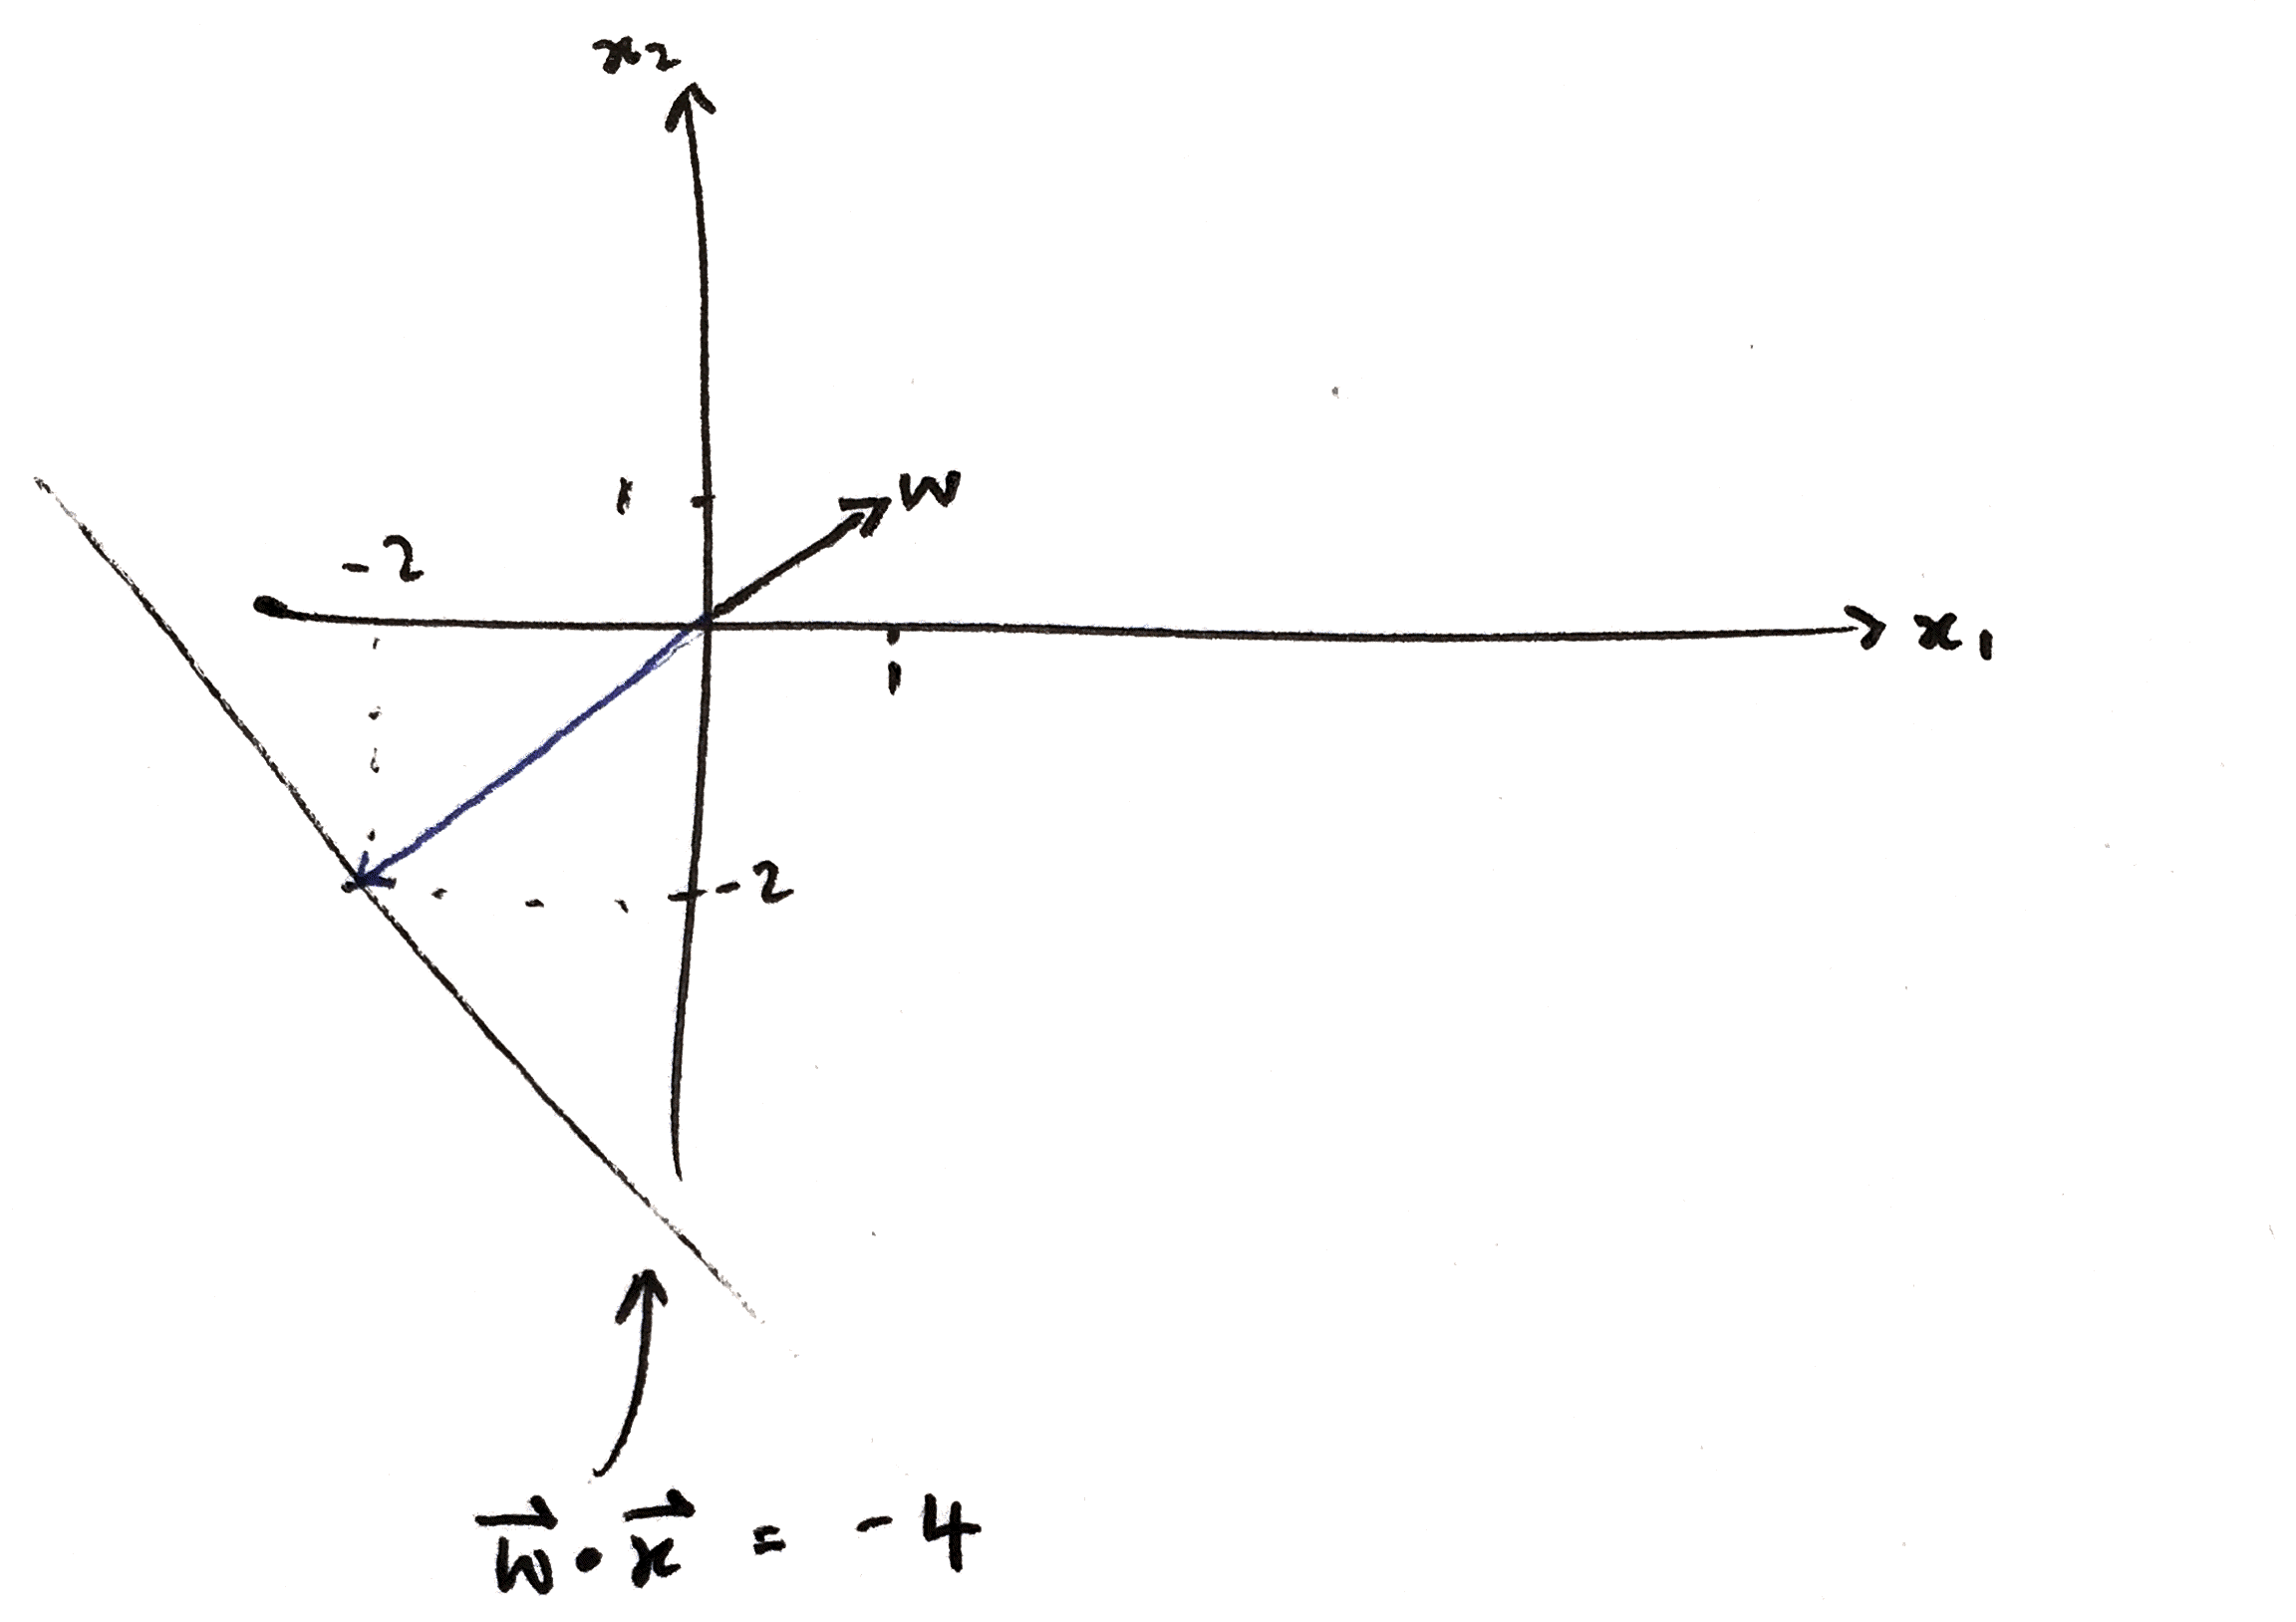
\includegraphics[width=200pt]{img/machine-learning-linear-decision-boundary.png}
\begin{itemize}
\item A plane sloping up at 45° in the north-east direction.
\item Each input feature has equal influence on the classification.
\item Decision boundary is line $x_1 + x_2 = -4$.
\item $\w$ is normal to the decision boundary since $\w \cdot (\x_1 - \x_2) = -4 - (-4) = 0$.
\item If one feature has a very high weight then $\w$ points close to that
  axis and the decision boundary is almost perpendicular to that axis (other
  features almost don't matter).
\end{itemize}

\textbf{Distance from the decision boundary to a point}: For some point $\x_i$,
the height of the decision function plane above $\x_i$ is
$\w \cdot \x_i + \alpha$. At the decision boundary, this height is
zero. Looking ``straight up'' the slope of the decision function, its gradient
is $\sqrt{w_1^2 + w_2^2} = |\w|$. So the distance of a point $\x_i$ from the
hyperplane is $\frac{\w \cdot \x_i + \alpha}{|\w|}$. If $\w$ is not a unit
vector, the problem can be rescaled so that it is, in which case the distance
is $\w \cdot \x_i + \alpha$.
\\
% \begin{mdframed}
%   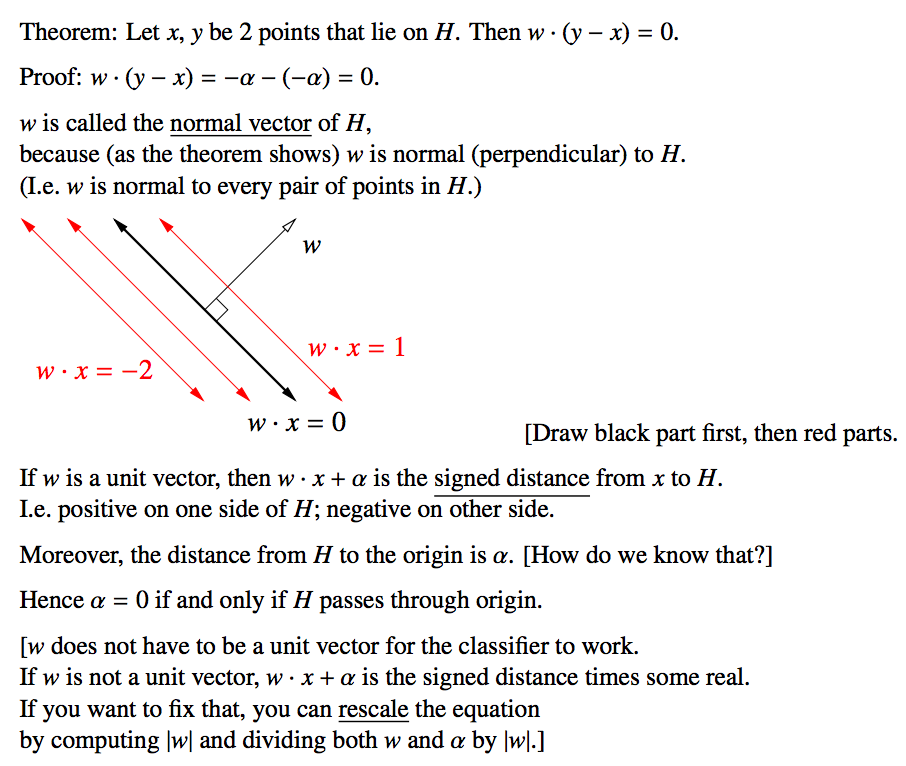
\includegraphics[width=300pt]{img/machine-learning-linear-decision-boundary-2.png}
% \end{mdframed}

\textbf{Examples of linear classifiers}:
\begin{itemize}
\item \textbf{Centroid method}:  Decision boundary perpendicular to and bisects line
  connecting means of labeled training points.
\item \textbf{Perceptron}:
\item \textbf{Maximum margin classifier}:
\item \textbf{LDA}:  Fit Gaussians to each class, same covariance across classes.
\end{itemize}

\subsection*{Perceptron}

Labels $y_i \in \{-1, 1\}$. Assume $\alpha=0$ for now (decision boundary through origin).

\textbf{Goal}: find line separating points (separating hyperplane). I.e. Find $\w$ such that
\begin{align*}
  \begin{cases}
    \x_i \cdot \w \leq 0, &y_i = -1 \\
    \x_i \cdot \w \geq 0, &y_i = +1.
  \end{cases}
\end{align*}
This is equivalent to the \textbf{constraint} $y_i\x_i \cdot \w \geq 0$.

\textbf{Cost function}: total distance $R(\w)$ of misclassified points from the
decision boundary.
\\
\begin{mdframed}
  \textbf{Optimization problem}: Find $\w$ that minimizes
  \begin{align*}
    R(w) = \sum_i L(\x_i \cdot \w, y_i) = \sum_{i \in V} -y_i\x_i \cdot \w,
  \end{align*}
  where $V$ are the misclassified points.
\end{mdframed}

Per-training point loss function
\begin{align*}
  L(\text{prediction}_i, y_i) = L(\x_i \cdot \w, y_i) =
  \begin{cases}
    0, &\text{correct}, y_i\x_i \cdot \w \geq 0\\
    -y_i\x_i \cdot \w, &\text{misclassified}
  \end{cases}
\end{align*}


\textbf{Gradient descent}: Find $w$ that minimizes $R(w)$.


\begin{align*}
  \nabla_w R = \cveccc{-\sum_i y_iX_{i1}}
                      {\vdots}
                      {-\sum_i y_iX_{id}}
\end{align*}
\begin{itemize}
\item On each iteration, compute the gradient; update $\w$ by taking a step
  downhill of size $\rho$: $\w \leftarrow \w + \rho \sum_{i \in V} y_i\x_i$.
\item A misclassified data point far out in dimension $j$ will cause the
  gradient to have a large component $-\sum_i y_iX_{ij}$ in that dimension.
\item $\w$ thus becomes more closely aligned with that axis and the decision
  boundary.
\item Decision boundary therefore becomes more perpendicular to that axis (axis
  becomes more ``important'').
\end{itemize}

\textbf{Stochastic gradient descent (Perceptron)}: on each iteration pick one misclassified
point and update $\w$ using gradient for that point:
$\w \leftarrow \w + \rho y_{i^*}\x_{i^*}$

\textbf{Allow decision boundaries that do not pass through origin}: add a
fictitious dimension so that sample points now lie on the plane $x_{d+1} = 1$
in $(d+1)$ dimensions. Run algorithm as above, just with the new
dimensionality.
\begin{align*}
  \w \cdot \x + \alpha &= 0 \\
  \cveccc{w_1}
         {w_2}
         {\alpha} \cdot \cveccc{x_1}{x_2}{1} &= 0.
\end{align*}

\subsection*{Optimization in weight space}

\begin{tabular}{l|l}
  $\x$-space    & $\w$-space \\
  \hline
  hyperplane & point $\w$ is normal vector to hyperplane \\
  point      & hyperplane whose normal vector is the $\x$ point (? don't understand this yet)
\end{tabular}

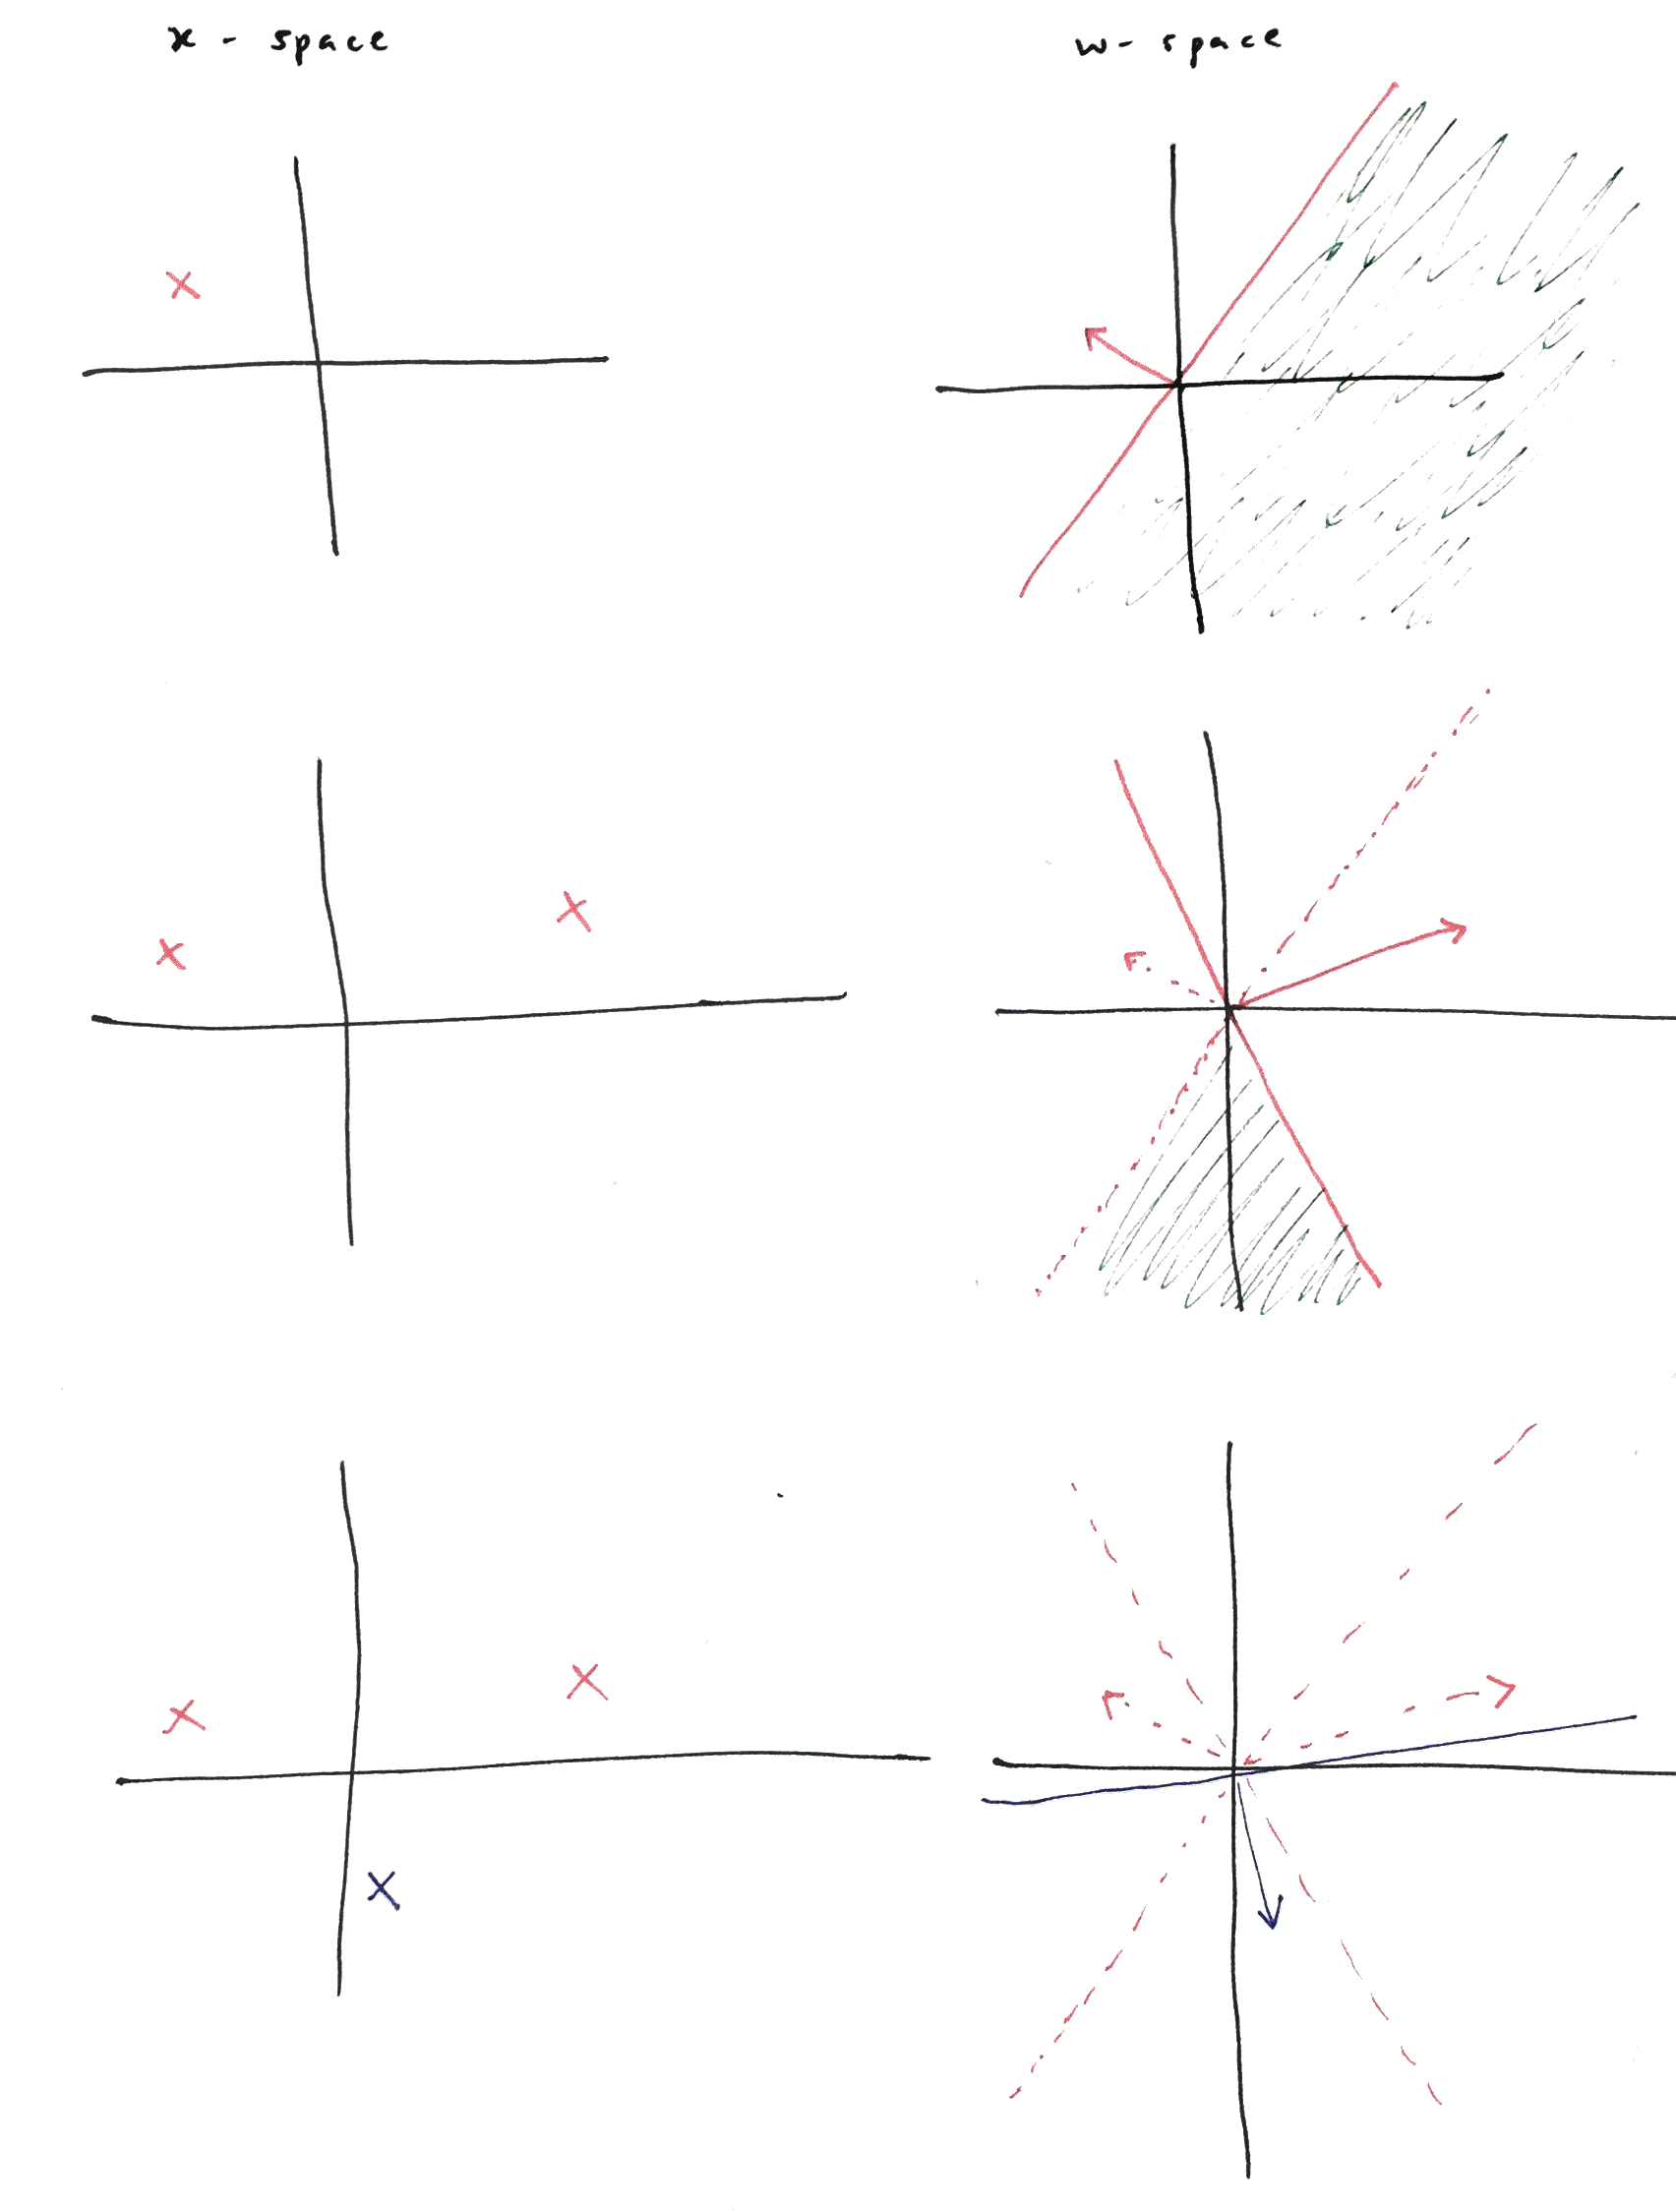
\includegraphics[width=200pt]{img/ml-perceptron-x-space-w-space.png}

\subsection*{Maximum margin classifiers}
\textbf{Margin} is distance from hyperplane to nearest sample point.

Previously, in the perceptron, we used the constraint
$$y_i \x_i \cdot \w \geq 0.$$
Now, we demand that there is a non-zero margin between the decision boundary
and the points:
$$y_i (\x_i \cdot \w + \alpha) \geq 1,$$
The 1 on the RHS is arbitrary; I think $\w$ and $\alpha$ will adapt to make it
true for any positive value, so the point is that we're demanding a strictly
non-zero margin.
\\
\begin{mdframed}
  \textbf{Optimization problem (quadratic program)}:\\
    Find $\w, \alpha$ that minimize $|\w|^2$ such that
    $y_i(\x_i \cdot \w + \alpha) \geq 1$ for all points $i$.
\end{mdframed}

\subsection*{Soft margin SVMs
\footnote{\url{https://people.eecs.berkeley.edu/~jrs/189/lec/04.pdf}}
\footnote{ \url{https://www.youtube.com/watch?v=HOZ6ZpPA_Ks}}
}

\begin{itemize}
\item Still quadratic program but allow points to violate margin via
  \textbf{slack variables} $\xi_i \geq 0$:
\item Constraint is $y_i(\x_i \cdot \w + \alpha) \geq 1 - \xi_i$
\item Find non-linear decision boundaries by introducing new features
  comprising non-linear functions of base features (``lift points into
  higher-dimensional space'').
\end{itemize}

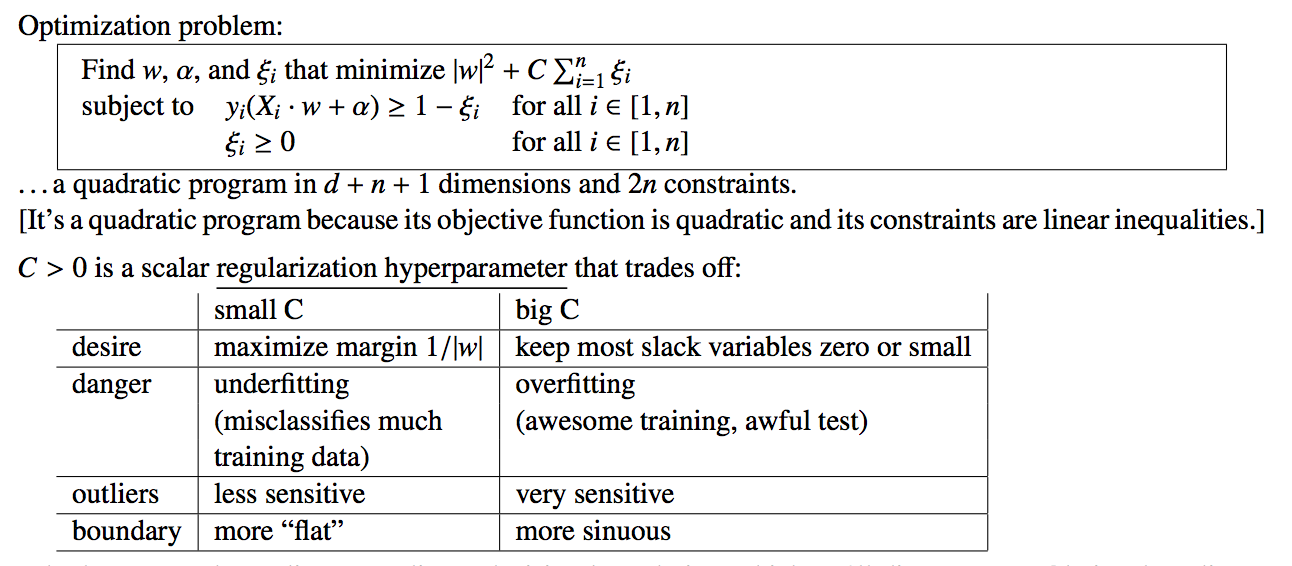
\includegraphics[width=300pt]{img/machine-learning-svm-1.png}
% 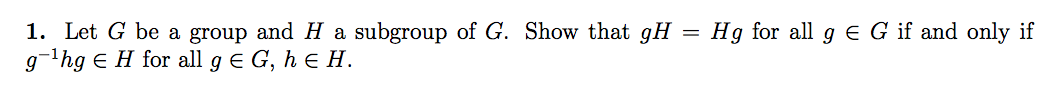
\includegraphics[width=300pt]{img/ml-svm-parabolic-lifting.png}



% \section*{5 Machine Learning Abstractions and Numerical Optimization}
% \url{https://people.eecs.berkeley.edu/~jrs/189/lec/05.pdf}\\
% \url{https://www.youtube.com/watch?v=DeIAXPUfCbQ}

\newpage
\section*{Decision Theory
  \footnote{\url{https://people.eecs.berkeley.edu/~jrs/189/lec/06.pdf}}
  \footnote{\url{https://www.youtube.com/watch?v=aXkenQ01qYI}}
}

Suppose there are two possible \textbf{classes}: $\{C, D\}$

\textbf{Decision rule}: $r(\x): \R^d \to \{C, D\}$

\textbf{Loss function}: E.g. 0-1 loss:
\begin{align*}
  L(y_i \to \hat y_i) =
  \begin{cases}
    0, & \hat y_i = y_i ~~~~~~~~~~~~~~~~~~~~\text{(correct classification)}\\
    1, & \otherwise
  \end{cases}
\end{align*}

\textbf{Risk}: Functional $R(r)$: expected loss for rule $r$, over $\p(X, Y)$.
\footnote{
\begin{align*}
  R(r) = &\pi(Y=-1)\E_\X L(-1 \to r(X)) + \\
         &\pi(Y=+1)\E_\X L(+1 \to r(X))~~~~~~~~~~~~~~~~~~~~~~~\text{over $\p(Y)\p(X|Y)$}
\end{align*}
\begin{align*}
  = \sum_X \p(X)\big(&\pi(Y=-1)L(-1 \to r(X)) + \\
                     &\pi(Y=+1)L(+1 \to r(X))\big)~~~~~\text{over $\p(X)\p(Y|X)$}
\end{align*}
}

So what rule function $r$ minimizes the functional $R$?

\textbf{Bayes decision rule}: Assign $\x$ to class $C$ if

\begin{center}
(C posterior at $\x$) $\times$ (penalty for misclassifing a true C)
\end{center}

is largest for class $C$. I.e. if
\begin{align*}
  \p(C|\x)L(D|C) > \p(D|\x)L(C|D).
\end{align*}

With 0-1 loss, this is: ``assign to class with highest posterior''.

With 0-1 loss and two classes, it's: ``assign to class with posterior $> 0.5$''.

\textbf{Empirical risk}: Discriminative methods (e.g. logistic regression) lack
any model for $X$. How can we estimate expected loss over $p(X,Y)$? Take the
observed sample points as defining a discrete, uniform distribution, in which
case
\begin{align*}
  \hat R(r) = \frac{1}{n}\sum L(r(x_i), y_i).
\end{align*}
This provides a justification for minimizing the sum/mean of per-sample loss.

\newpage
\section*{Statistical justifications}

Regression: want to estimate a function $f$ such that
$y_i = f(x_i) + \epsilon$, where $\epsilon$ has unknown distribution but mean
0. Ideal would be to estimate $f$ with $h(x_i) = \E(Y|x_i)$ since this is equal
to $f(x_i)$.

Likelihood justification for linear regression cost function.

Logistic Regression from Maximum Likelihood

\section*{Bias-Variance Decomposition}

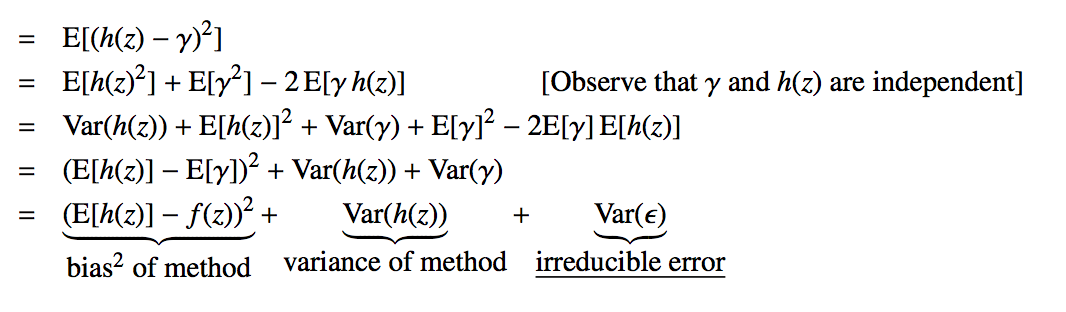
\includegraphics[width=300pt]{img/machine-learning-bias-variance-decomp-1.png}





\newpage
\section*{Gaussian discriminant analysis
  \footnote{\url{https://people.eecs.berkeley.edu/~jrs/189/lec/07.pdf}}
  \footnote{\url{https://www.youtube.com/watch?v=4CefboCXxZs}}
}

\textbf{Anisotropic}:
\begin{align*}
  \p(\x) = \frac{1}{(2\pi)^{d/2}|\Sigma|^{1/2}} \exp\(-\frac{1}{2}(\x - \mu)^\T\Sigma^\1(\x - \mu)\)
\end{align*}

\textbf{Isotropic}:
\begin{align*}
  \p(\x) = \frac{1}{(2\pi)^{d/2}\sigma^d} \exp\(-\frac{|\x - \mu|^2}{2\sigma^2}\)
\end{align*}

\newcommand{\class}{\text{class~}}

\subsection*{Isotropic Gaussians}

Multivariate data $\x$ but features uncorrelated and all features same variance.L

\subsubsection*{QDA}
Fit separate Gaussians to the training data in each class. The likelihood is
\begin{align*}
  \p(\x|\class C) = \frac{1}{(2\pi)^{d/2}\sigma_C^d}\exp\(-\frac{|\x - \mu_C|^2}{\sigma_C^2}\)
\end{align*}

and we compare the value of $\p(\x|\class C) \cdot \pi_C \cdot L(D|C)$.

The decision boundaries are where the posterior $\times$ loss are equal. It's
easier to compare the log of this:
\begin{align*}
  Q_C(\x) = - \frac{|\x - \mu_C|^2}{\sigma_C^2} - d\log \sigma_C + \log \pi_C + \log L(D|C)
\end{align*}

\begin{comment}
  So the decision boundary is at $\x$ satisfying
  \begin{align*}
    Q_C(\x) - Q_D(\x) &= 0 \\
    \frac{|\x - \mu_D|^2}{\sigma_D^2} - \frac{|\x - \mu_C|^2}{\sigma_C^2} +
    d\log \frac{\sigma_D}{\sigma_C} +
    \log \frac{\pi(C)}{\pi(D)} +
    \log \frac{L(D|C)}{L(C|D)}
     &= 0 \\
  \end{align*}
\end{comment}

The posterior probability of class $C$ at point $\x$ is\footnote{This is
  assuming 0-1 loss, so the loss doesn't affect $Q_C(\x)$}
\begin{align*}
  \p(C|\x)
  = \frac{\pi_C\p(\x|C)}{\pi_C\p(\x|C) + \pi_D\p(\x|D)}
  = \frac{1}{1 + e^{-(Q_C(\x) - Q_D(\x))}},
\end{align*}
so logistic in the quadratic expression $Q_C(\x) - Q_D(\x)$.

\subsubsection*{LDA}
Estimate separate class means but same variance for all classes. So now
\begin{align*}
  Q_C(\x) - Q_D(\x)
  &= \frac{|\x - \mu_D|^2 - |\x - \mu_C|^2}{\sigma^2} + \log \frac{\pi_C}{\pi_D} + \log \frac{L(D|C)}{L(C|D)} \\
  &= \frac{(\x - \mu_D)\cdot(\x - \mu_D) - (\x - \mu_C)\cdot(\x - \mu_C)}{\sigma^2} + \log \frac{\pi_C}{\pi_D} + \log \frac{L(D|C)}{L(C|D)} \\
% &= \frac{ 2(\x\cdot\mu_C - \x\cdot\mu_D) + |\mu_D|^2 - |\mu_C|^2}{\sigma^2} + \log \frac{\pi_C}{\pi_D} + \log \frac{L(D|C)}{L(C|D)} \\
  &= \x\cdot\frac{2(\mu_C - \mu_D)}{\sigma^2} + \(\frac{|\mu_D|^2 - |\mu_C|^2}{\sigma^2} + \log \frac{\pi_C}{\pi_D} + \log \frac{L(D|C)}{L(C|D)}\) \\
  &= \x\cdot\w + \alpha
\end{align*}
This means that the decision boundary is linear, and (with 0-1 loss) the
posterior is a logistic function which is constant parallel to the decision
boundary.

\section*{Symmetric matrices, quadratic forms and eigenvectors
  \footnote{\url{https://people.eecs.berkeley.edu/~jrs/189/lec/08.pdf}}
}

\textbf{Spectral theorem}: A symmetric matrix has $n$ \textbf{orthogonal}
eigenvectors\footnote{There may be more than $n$ (infinite) eigenvectors, but
  $n$ orthogonal.}\footnote{Non-symmetric matrices have non-orthogonal eigenvectors in
  general.}


To understand a symmetric matrix $\A$, consider its \textbf{quadratic form}
$|\A\x|^2 = \x^\T \A^2\x$ (right). Compare this to the graph of $|\z|^2$
(left). The graphs are related by the following changes of coordinates:

$\z \gets \A\x$ changes the elliptical contours into circles; scale by eigenvalues of $\A$.

$\A^\1 \z \to \x$ changes circles into ellipses; scale by reciprocal of eigenvalues.

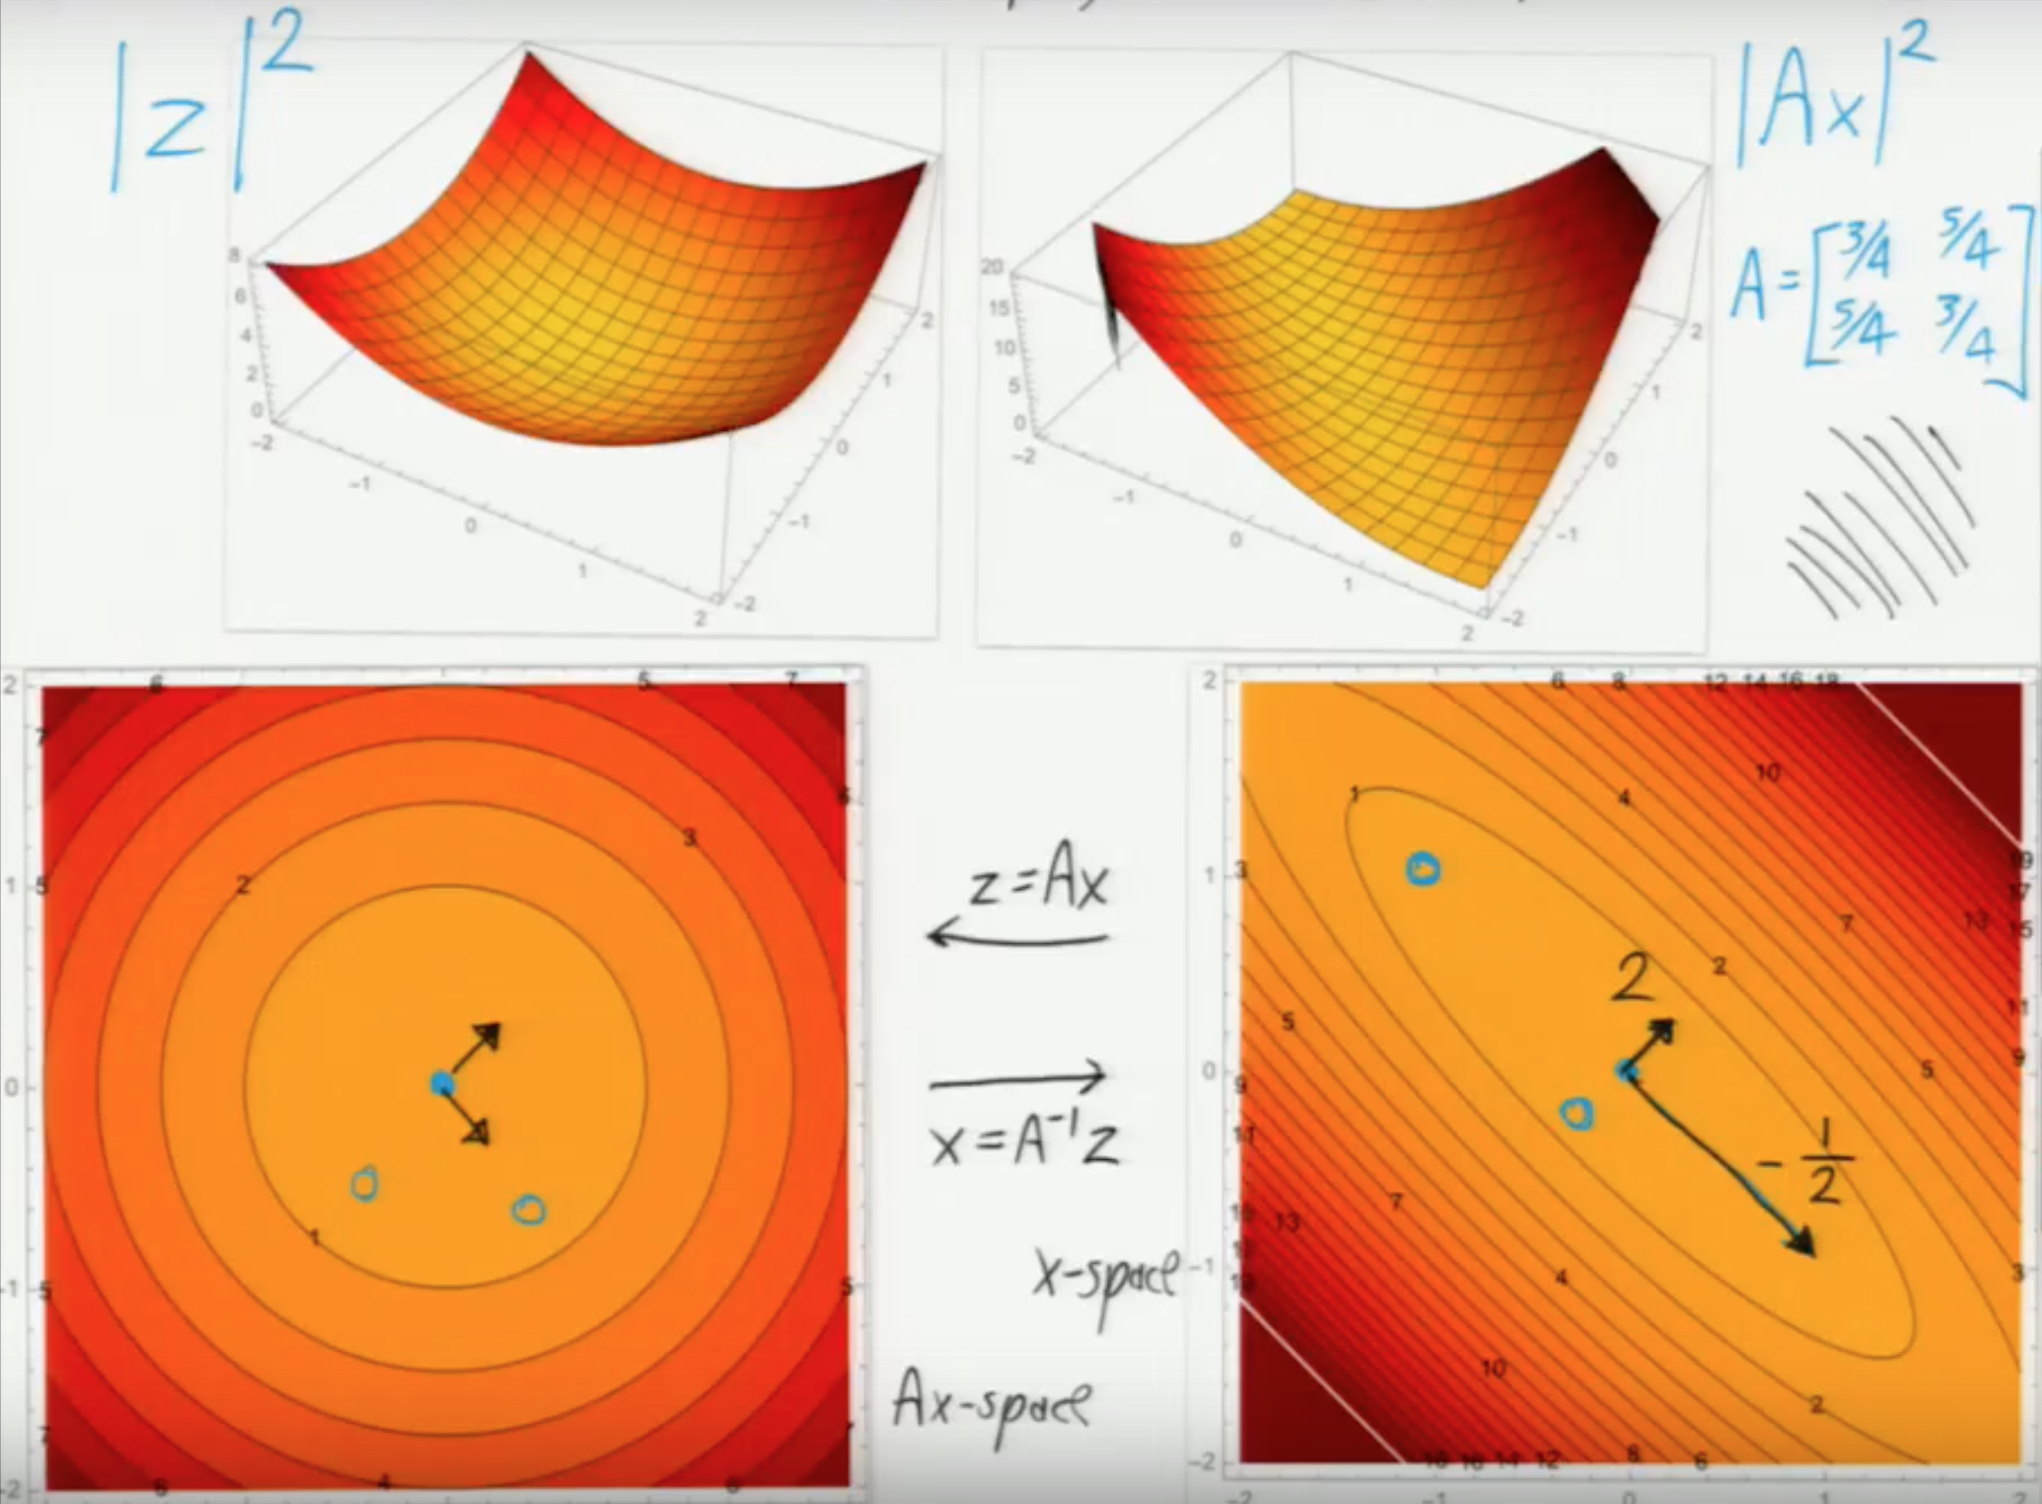
\includegraphics[width=300pt]{img/machine-learning-quadratic-form-eigenvectors.png}

$|\A\x|^2 = 1$ is the equation of an ellipsoid. Its axes are $v_1,\ldots,v_n$
and its radii are $\frac{1}{\lambda_1},\ldots,\frac{1}{\lambda_n},$

Bigger eigenvalue $\iff$ steeper hill.

Alternate interpretation: the ellipsoids are spheres in a space with a
different distance metric. The distance metric (metric tensor) is $\mat M=\A^2$:
\begin{align*}
  d(\x,\x') = |\A\x| - |\A\x'| = \sqrt{(\x - \x')\A^2(\x - \x')}
\end{align*}


\begin{minipage}{\textwidth}
These are diagrams of $\x^\T\A\x$ (not $\x^\T\A^2\x$ since $\A^2$ has no negative eigenvalues):

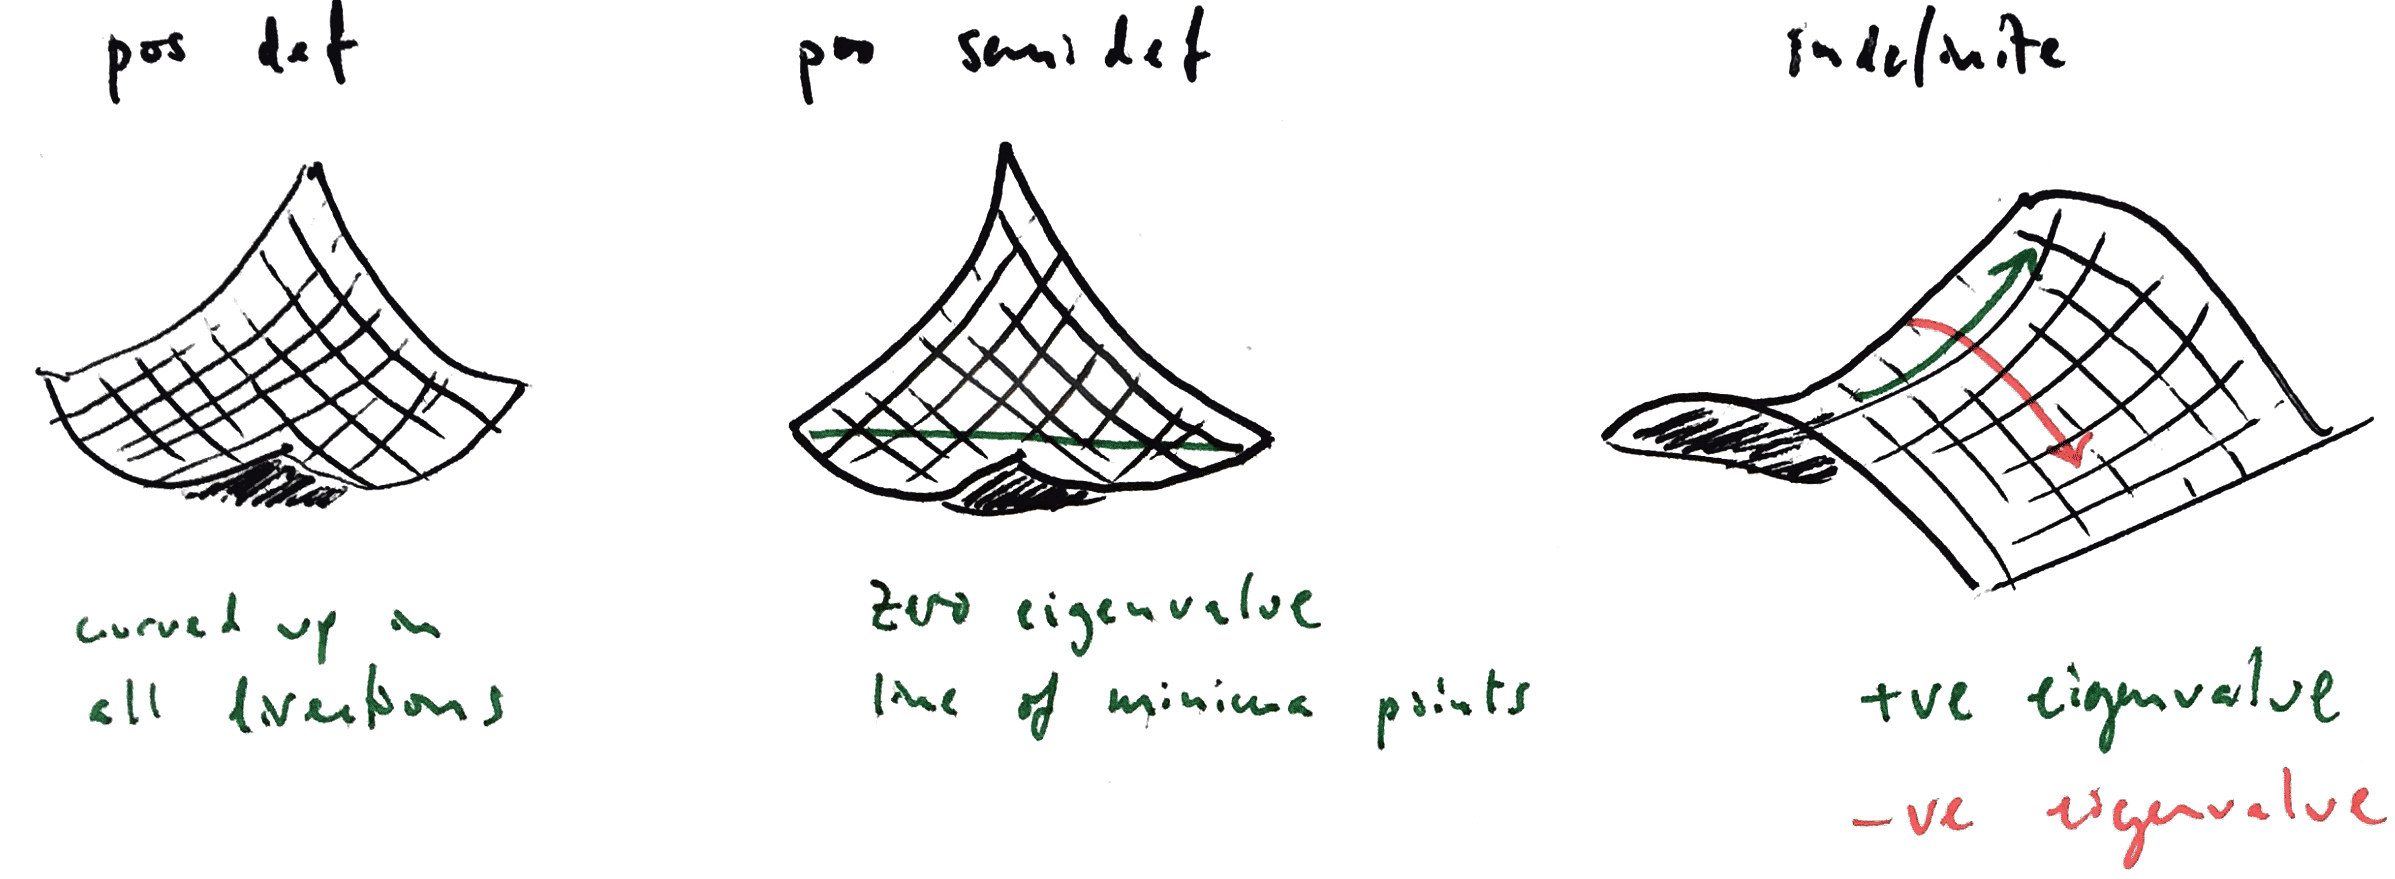
\includegraphics[width=300pt]{img/machine-learning-quadratic-form-eigenvectors-2.png}

\begin{tabular}{ l | l | l }
  \textbf{positive definite}     & eigenvalues $> 0$    & $\x^\T\A\x > 0 ~~~~~~ \forall \x \neq \0$ \\
  \textbf{positive semidefinite} & eigenvalues $\geq 0$ & $\x^\T\A\x >= 0 ~~~~ \forall \x$ \\
  \textbf{indefinite}            & some positive and some negative eigenvalues & \\
  \textbf{singular}              & some zero eigenvalue \\
\end{tabular}
\end{minipage}

Let $\Lambda$ be a diagonal matrix containing the eigenvalues and $\V$ contain
normalized eigenvectors:
\begin{align*}
V = \begin{bmatrix}
\mid & \mid & & \mid \\
\v_1 & \v_2 & \cdots & \v_n\\
\mid & \mid & & \mid \\
\end{bmatrix}
\end{align*}

Note that for an \textbf{orthonormal} matrix like this:
\begin{enumerate}
\item It rotates / reflects the input vectors, without changing their length.
\item  $\V^T\V = \I$, therefore $\V^\1 = \V^\T$.
\end{enumerate}


By the definition of eigenvector we have
\begin{align*}
  \A\V = \V\Lambda
\end{align*}
and therefore the \textbf{eigendecomposition} of $\A$
\begin{align*}
  \A = \V\Lambda\V^\T.
\end{align*}

So we can perform $\A\x$ as $\V\Lambda\V^\T\x$, and $\A^k\x$ as
$\V\Lambda^k\V^\T\x$:

\begin{enumerate}
\item $\V^\T = \V^\1$ rotates the input vector into axis-aligned coordinates.
\item $\Lambda$ scales along different axes.
\item $\V$ returns to the original coordinates.
\end{enumerate}

$\Lambda$ is said to be the diagonalized version of $\A$.
\section*{9 The Anisotropic Multivariate Normal Distribution, QDA, and LDA}

\newpage
\section*{Regression}
\subsection*{Linear Least Squares Regression}
Use fictitious dimension trick, so that $\w$ includes the offset term $\alpha$
and $\X$ is $(n \times (d + 1))$.
\\
\begin{mdframed}
Find $\w$ that minimizes cost function $J(w)$: sum of squared difference between
linear predictor and observed training point.
\begin{align*}
  J(w) = |\X \w - \y|^2 = \sum_i (\x_i^\T\w - y_i)^2
\end{align*}
\end{mdframed}

Solve by differentiating and finding the critical point:
\begin{align*}
  |\X \w - \y|^2          &= \w^\T\X^\T\X\w - 2\y^\T\X\w + \y^\T\y \\
  \grad_\w |\X \w - \y|^2 &= 2 \X^\T\X\w - 2\X^\T\y \\
  \w^*                    &= (\X^\T\X)^{-1}\X^\T\y =: \X^+\y
\end{align*}
\begin{mdframed}
For a new sample point $\x$, the prediction is $\hat y = \x \cdot \w^*$.
\end{mdframed}

\subsubsection*{Related concepts}
\begin{itemize}
\item \textbf{normal equations}: linear system of $d$ equations in unknown $\w$ resulting from
  setting the gradient equal to zero: $\X^\T\X\w - \X^\T\y = \vec 0$
\item \textbf{pseudoinverse}: The matrix $\X^+ = (\X^\T\X)^{-1}\X^\T$ maps $\y$
  to $\w^*$. In general there's no $\w$ that solves $\X\w = \y$, but
  $\w^* = \X^+\y$ makes the LHS as close as possible to $\y$. So it behaves as
  a ``left inverse'' of $\X$, since $\X^+\X = \I$ and left-multiplying by $\X^+$
  gives the ``solution'' to $\X\w = \y$.
\item \textbf{projection matrix} or \textbf{hat matrix}: Still focusing on the
  training phase, the predictions are $\hat \y = \X\w^* = \X\X^+\y$. So
  $\X\X^+$ puts that hat on $\y$, or projects $\y$ onto the hyperplane, in the
  viewpoint described below.
\end{itemize}

\subsubsection*{Projection interpretation}
Usually we think of $n$ points in $\R^d$. But instead, consider a separate
column of the data for each feature: these are $d$ points in $\R^n$. The
observed training data $\y$ is also a point in $\R^n$, and so is the prediction
$\hat \y = \X\w$.

As we vary $\w$, the prediction $\X\w$ describes a hyperplane spanned by the
columns of $\X$.

We want to find the $\w^*$ corresponding to the closest point on the hyperplane
to $\y$. So $X\w^* - \y$ must be orthogonal to the hyperplane:
\begin{align*}
  \X^\T \cdot (\X\w^* - \y) = \vec 0.
\end{align*}
Which are the normal equations (linear system of $d$ equations), derived
differently.

\subsubsection*{Weighted linear regression}
Sample point $i$ has weight $b_i$. Diagonal $n \by n$ matrix $\mat B$ contains weights.
\begin{align*}
  J(\w) &= \sum_i b_i (\x_i^\T\w - y_i)^2 \\
        & = (\X\w - \y)^\T \B (\X\w - \y) \\
        &= \w^\T\X^\T \B \X\w - 2\y^\T \B \X\w + \y^\T\y
\end{align*}
Gradient
\begin{align*}
  \grad_\w J(\w) = 2\X^\T \B \X\w - 2\X^\T\B\y
\end{align*}
Solution
\begin{align*}
  \w^* = \(\X^\T \B \X\)^{-1}\X^\T\B\y
\end{align*}

\subsubsection*{How to compute the gradient}

The cost function is $J(\w) = |\X\w - \y|^2$. We could write this as a dot product and
multiply out:
\begin{align*}
  J(\w) &= (\X\w - \y) \cdot (\X\w - \y) \\
  &= \X\w \cdot \X\w - 2 \X\w \cdot \y + \y \cdot \y \\
  &= (\X\w)^\T \X\w - 2 (\X\w)^\T \y + \y^\T \y \\
  &= \w^T\X^\T\X\w - 2 \w^\T\X^\T\y + \y^\T \y,
\end{align*}
and then we'd need to differentiate those terms w.r.t. $\w$. However, a better
way is to use the chain rule. Define $f$ and $g$ such that
$J: \R^d \rightarrow \R$ is their composition $J = g \circ f$:
\begin{align*}
  &f: \R^d \rightarrow \R^n     &f(\w) = \X\w - \y \\
  &g: \R^n \rightarrow \R       &g(\vec z) = |\vec z|^2.
\end{align*}
The chain rule says that $\grad (g \circ f) = (D f)^\T \grad g$, where $D f$ is
the derivative of $f$, i.e. the Jacobian matrix of first partial
derivatives\footnote{The gradient $\grad$ applies only to scalar-valued
functions.}. We have $D f(\w) = \X$ and $\grad g(\z) = 2\z$, so
\begin{align*}
  \grad J(\w)
  &= 2\X^\T(\X\w - \y) \\
  &= 2\X^\T\X\w - 2\X^\T\y.
\end{align*}

\subsection*{Penalized Regression}
TODO

\subsection*{Logistic Regression}

\begin{itemize}
\item Two classes.
\item The observations $y_i$ are class labels (or probabilities thereof).
\item The model states that the probability of being in class 1 is given by the
  usual linear model, mapped onto $(0, 1)$ by the logistic function $s$:
  $$y_i \sim \Bern(s(\x_i^\T\w)),$$
  $$s(z) = \frac{1}{1 + e^{-z}}$$
\end{itemize}
Note that $s'(z) = \frac{e^{-z}}{(1 + e^{-z})^2} = s(z)(1 - s(z))$.

\subsubsection*{Likelihood}
Let $s_i = s(\x_i^\T\w)$.
\begin{align*}
  \L(\w)       &= \prod_i s_i^{y_i} + \(1 - s_i\)^{(1 - y_i)} \\
  \l(\w)       &= \sum_i y_i \log s_i + (1 - y_i) \log\(1 - s_i\) \\
\grad \l(\w) &= \sum_i \frac{y_i}{s_i}(s_i)(1 - s_i)\x_i + \frac{1 - y_i}{1 - s_i}(-1)(s_i)(1 - s_i)\x_i \\
             &= \sum_i \x_i\(y_i(1 - s_i) - (1 - y_i)s_i\) \\
             &= \sum_i \x_i\(y_i - s_i\) \\
             &= \X^\T\(\y - \s(\X\w)\) ~~~~~~~~~ (d \by 1)
\end{align*}

where $\s: \R^n \to \R^n$ applies $s$ componentwise to the rows.

\textbf{Optimization problem}: Find $\w$ that minimizes the cost function
$J(\w) = -\l(\w)$.

Because the weights $\w$ are tied up inside $s_i = s(\x_i^\T\w)$ it's not
possible to find the minimum $\w^*$ by setting the gradient equal to zero
(i.e. by solving a linear system). We can use gradient descent, or Newton's
method.

For Newton's method, we need the Hessian of the objective function. This is the
$d \by \d$ matrix of partial derivatives of the gradient, i.e. $\X^\T$
multiplied by the derivative (Jacobian matrix) of $\s(\X\w)$. Define
$\f(\w) = \X\w$ so now $\s(\X\w) = (\s \circ \f)(\w)$.

\begin{tabular}{l | l | l | l}
  Function         & domain $\to$ range    & Jacobian                               & dim Jacobian \\
  \hline
  $\f(\w) = \X\w$  &$\R^d \rightarrow \R^n$ &$\D\f = \X$                            & $n \by d$\\
  $\s(\z)$         &$\R^n \rightarrow \R^n$ &$\D\s(\z) = \S$ & $n \by n$
\end{tabular}

where $\S$ is a diagonal matrix with
$\S_{ii} = \s(\x_i^\T\w)(1 - \s(\x_i^\T\w))$. Now by the chain rule,
\begin{align*}
%\D_\w \s(\X\w) &= \D_\w \s(\f(\w)) = ((\D_f \s) (\D_\w \f))(\w) = \s(\f(\w))(1 - \s(\f(\w)))^\T \X
\hess J(\w) &= \X^\T \D_\w \s(\X\w) \\
            &= \X^\T (\D_\f \s) (\D_w \f) \\
            &= \X^\T\S\X.
\end{align*}



% \section*{11 More Regression; Newton’s Method; ROC Curves}

\section{ Change of basis}

Suppose person B uses some other basis vectors to describe locations in
space. Specifically, in our coordinates, their basis vectors are
$\scvec{2}{1}$ and $\scvec{-1}{1}$.


\textbf{When they state a vector, what is it in our coordinates?}

If they say $\scvec{-1}{2}$, what is that in our coordinates?

Well, if they say $\scvec{1}{0}$, that's $\scvec{2}{1}$ in our coordinates. And
if they say $\scvec{0}{1}$, that's $\scvec{-1}{1}$ in our coordinates. So the
matrix containing \textit{their basis vectors expressed using our coordinate system}
transforms a point expressed in their coordinate system into one expressed in
ours. That last sentence is critical, so hopefully it makes sense! So, the answer is

$$
\mat{2}{-1}
    {1}{ 1} \cvec{-1}{2} = \cvec{-4}{1}.
$$


\textbf{When we state a vector, what is it in their coordinates?}

We give the vector $\scvec{3}{2}$. What is that in their coordinate system? By
definition, the answer is the weights that scales their basis vectors to hit
$\scvec{3}{2}$. So, the solution to

$$
\mat{2}{-1}
    {1}{1} \cvec{a}{b} = \cvec{3}{2}.
$$


Computationally, we can see that we can get the solution by multiplying both
sides by the inverse:

$$
\cvec{a}{b} = \mat{2}{-1}
                  {1}{1}^{-1} \cvec{3}{2}.
$$

Conceptually, we have

$$
\mat{2}{-1}
    {1}{1} =
\begin{bmatrix}\text{matrix converting their}\\\text{representation to ours} \\ \end{bmatrix}
$$

where "their representation" means the vector expressed using their coordinate
system. So the role played by the inverse is

$$
\cvec{a}{b} =
\begin{bmatrix}\text{matrix converting our}\\\text{representation to theirs} \\ \end{bmatrix}
\cvec{3}{2}.
$$

\textbf{When we state a transformation, what is it in their coordinates?}

We state a 90° anticlockwise rotation of 2D space:

$$
\mat{0}{-1}
    {1}{0}
$$

what is that transformation in their coordinates? The answer is

$$
\begin{bmatrix}\text{matrix converting our}\\\text{representation to theirs} \\ \end{bmatrix}
\mat{0}{-1}
    {1}{0}
\begin{bmatrix}\text{matrix converting their}\\\text{representation to ours} \\ \end{bmatrix}
$$

since the composition of those three transformations defines a single
transformation that takes in a vector expressed in their coordinate system,
converts it to our coordinate system, transforms it as requested, and then
converts back to theirs.


\section{Symmetric matrices}

\textbf{Spectral theorem for symmetric matrices}

Symmetric $n \by n$ matrix $A$ (real).

$A^\1 = A^\T$

$n$ orthogonal eigenvectors with real eigenvalues.

Orthonormal matrix $U$ containing normalized eigenvectors.

$A = U\Lambda U^\1 = U\Lambda U^\T$

(Eigenvalues are uniquely determined by matrix. Eigenvalues can be repeated, in which case any linear combination of their
eigenvalues is also an eigenvalue.)



\section*{Linear and quadratic approximations to a function
  \footnote{
    \href{https://www.khanacademy.org/math/multivariable-calculus/applications-of-multivariable-derivatives/optimizing-multivariable-functions/a/reasoning-behind-the-second-partial-derivative-test}{khanacademy - Grant Sanderson - second partial derivative test}
  }
}



We construct first- and second-order approximations to a differentiable
function $f: \R^2 \rightarrow \R$. The approximation is made at some point
$(x_0, y_0) = \vec x_0 \in \R^2$; we demand that the value of the approximation, and the
first and second derivatives, match those of $f$ exactly at that point.

\subsection*{Linear approximation to a function $f(x, y)$ near $(x_0, y_0)$:}

\begin{align*}
L(x, y) &=
~
f(x_0, y_0) ~+
(x - x_0)f_x(x_0,y_0) +
(y - y_0)f_y(x_0,y_0)
\\\\
&= f(\vec x) + (\vec x - \vec x_0) \cdot \nabla_f(\vec x_0)
\end{align*}

Note that, at $(x_0, y_0)$, the first partial derivatives of $L$ are equal to
those of $f$, as they must be. (In fact, we could say that the coefficients are
determined by this requirement; see the quadratic case below. But the linear
case is obvious without ``deriving'' the coefficients.)


\subsection*{Quadratic approximation to a function $f(x, y)$ near $(x_0, y_0)$:}

First note that the ``quadratic form'' $ax^2 + 2bxy + cy^2$ can be written as
\begin{align*}
\x^\T A \x = \cvec{x}{y}^\T \mat{a}{b}
                                {b}{c} \cvec{x}{y}.
\end{align*}
This is a scalar. In general, a quadratic form for symmetric matric $A$ is
\begin{align*}
\x^\T A \y = \sum_{jk}A_{jk}x_jy_k.
\end{align*}

The $j$-th component of the gradient of $q(\x) = \x^\T A \x$ is
$\partiald{q}{x_j} = 2\sum_k A_{jk}x_k$, so
\begin{align*}
  \nabla ~\x^\T \vec A \x = 2\vec A \x.
\end{align*}

\begin{align*}
Q(x, y) &=
f(\vec x_0) + (x - x_0)f_x(\vec x_0) +
(y - y_0)f_y(\vec x_0) ~+ \\
&~~~~~~~\frac{1}{2} f_{xx}(\vec x_0)(x - x_0)^2 +
f_{xy}(\vec x_0)(x - x_0)(y - y_0) +
\frac{1}{2} f_{yy}(\vec x_0)(y - y_0)^2 \\\\
&= f(\vec x_0) +
(\vec x - \vec x_0) \cdot \nabla f(\vec x_0) +
\frac{1}{2}(\vec x - \vec x_0)^\T \nabla^2 f(\vec x_0)(\vec x - \vec x_0),
\end{align*}
where $\nabla^2 f(\vec x_0)$ is the Hessian matrix $\mat{f_{xx}}{f_{xy}}
                                                        {f_{yx}}{f_{yy}}$ evaluated at $\vec x_0$.

\subsection*{Second partial derivative test and positive definiteness of Hessian}

The second partial derivative test for a function of two variables states that
we examine the determinant of the Hessian evaluated at the critical point:
$$
D = \det \nabla^2 f(\vec x_0) = f_{xx}(\vec x_0)f_{yy}(\vec x_0) - f_{xy}(\vec x_0)^2.
$$

Notice that $D \geq 0$ implies that the sign of $f_{xx}$ and $f_{yy}$ agree
(because we're subtracting the square of the mixed partial $f_{xy}$, i.e. a
positive number).

\begin{tabular}{ l l l l l }
  $D$    & roots          & $f_{xx}$ &  & Hessian \\
  \hline
  $+$    & no real roots  & $+$     & minimum        & positive definite \\
  $+$    & no real roots  & $-$     & maximum        & negative definite \\
  $0$    & one real root  & $+$     & minimum        & positive semidefinite \\
  $0$    & one real root  & $-$     & maximum        & negative semidefinite \\
  $-$    & two real roots & n/a     & saddle point   & - \\
\end{tabular}

\subsubsection*{Explanation}
At a critical point $\vec x_0$, the gradient is zero and the quadratic approximation is therefore
$$
Q(x, y) = f(\vec x_0) + \frac{1}{2}(\vec x - \vec x_0)^\T \nabla^2 f(\vec x_0)(\vec x - \vec x_0).
$$
So if this is a minimum (concave-up paraboloid) then this quadratic form is
positive for all $\vec x \neq \vec x_0$ (and if it's a maximum then it's
negative for all $\vec x \neq \vec x_0$).

Basically the argument is that, instead of analyzing the function $f$ itself,
we analyze its quadratic approximation at the critical point. So the question
comes down to: how do we determine whether a quadratic form is always positive,
always negative, or takes positive and negative values?

To answer that, consider a generic quadratic form $ax^2 + 2bxy + cy^2$. Let $y$
be constant at $y_0$; then we have a quadratic in $x$, the roots of which are
\begin{align*}
  x
  = \frac{-2by_0 \pm \sqrt{4b^2y_0^2 - 4acy_0^2}}{2a}
  = y_0\frac{-b \pm \sqrt{b^2 - ac}}{a}.
\end{align*}
So, whether this is a saddle point or a minimum/maximum depends on whether the
quadratic form has real roots. If there are no real roots, then whether it's a
minimum or a maximum depends on the sign of $f_{xx}$ (this sign will be the
same as that of $f_{yy}$ in the no real roots case).


\end{document}
